%%%%%%%%%%%%%%%%%%%%%%%%%%%%%%%%%%%%%%%
%                                                                              
% 		Management- und Dokumentationsattribute 			      		
%                                                                              
%%%%%%%%%%%%%%%%%%%%%%%%%%%%%%%%%%%%%%%

TODO Einleitung Management- und Dokumentationsattribute\\
\scalebox{0.45}{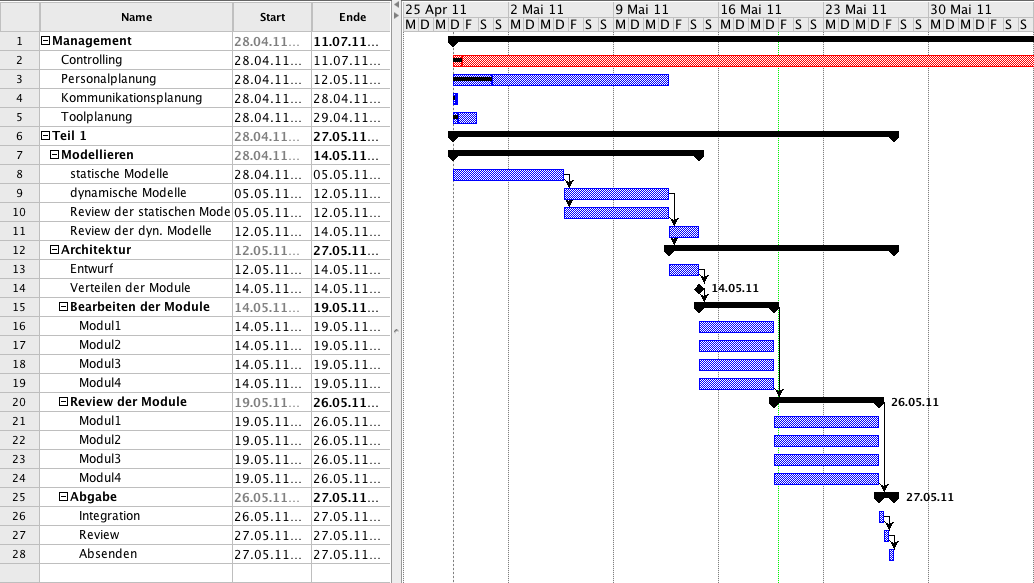
\includegraphics{data/fig/ganth_beispiel.png}}
Die Managementattribute des Softwareprodukts und dessen Anforderungen, werden anfangs mit Initialwerten samt Wertebereich versehen:\\
\ \\
Priorität aus Auftraggebersicht = {hoch, mittel, niedrig}\\
Priorität aus Auftragnehmersicht = {hoch, mittel, niedrig}\\
Stabilität = {fest, gefestigt, volatil}\\
Kritikalität = {hoch, mittel, niedrig, keine}\\
Entwicklungsrisiko = {hoch, mittel, niedrig}\\

\subsection{Dokumentationsattribute}
Autor	
Eindeutige Teamnummer	
Quelle	
Version	
Bearbeitungsstatus	

\subsection{Managementsattribute}
\begin{itemize}
	\item[] Managementattribute
	\item[] Priorität
	\item[]	Stabilität
	\item[] Kritikalität	
	\item[] Entwicklungsrisiko
\end{itemize}

